%
%  Chapter:  3 - 135Pr Experimental Methods
%  Modified: 2/16/2015
%  Author:   James Till Matta
%
%%%%%%%%%%%%%%%%%%%%%%%%%%%%%%%%%%%%%%%%%%%%%%%%%%%%%%%%%%

\chapter{EXPERIMENTAL METHODS}
\label{chp:exp-pr}
Across all of experimental physics there is a common theme in the design of an experiment. Finding a way of producing the system to be studied is one part of this theme. The other part is having the equipment to collect the signals necessary to understand what the system is doing. In nuclear physics, the appropriate choice of reaction will create the desired system and the equipment for signal collection will depend greatly on what one wishes to measure. This chapter will discuss the reaction, detectors, and techniques used in the examination of transverse wobbling in \pr{}.
\section{Heavy-ion Fusion-evaporation Reaction}
\label{sec:exp-pr-fus-evap}
Across nuclear physics there are vast array of reactions used. Narrowing to in-beam \gr{} spectroscopy one finds some common ``workhorse'' reactions that are commonly used. Of these workhorse reactions the heavy-ion fusion-evaporation reaction is frequently chosen for its selectivity in final products, producing relatively few species with large cross-section, and its creation of states with a large amount of angular momentum.\cite{beausang1996arrays}.
\subsection{Creation and Decay of the Compound Nucleus}
\label{ssec:exp-pr-fus-evap-cn}
The fusion evaporation reaction proceeds by the formation of a highly excited compound nucleus\cite{bohr1936neutron}, followed by the evaporation of particles, finally leaving behind the excited residual nucleus. In the particle evaporation process each particle must penetrate a barrier, for neutrons this barrier is merely the centrifugal barrier while charged particles see the coulomb barrier as well, this makes neutron emission more probable. Each successive evaporated particle carries energy away from the nucleus until there is insufficient excitation energy for particles to penetrate the emission barrier and the nucleus is left in a state that is stable against particle emission. From this point on the nucleus must dissipate its excess angular momentum and excitation energy via \gr{} emission. A schematic of a (HI, $p3n\gamma{}$) reaction is shown in Fig. \ref{fig:chp3-fus-evap-schem}.
\begin{figure}
	\centerline{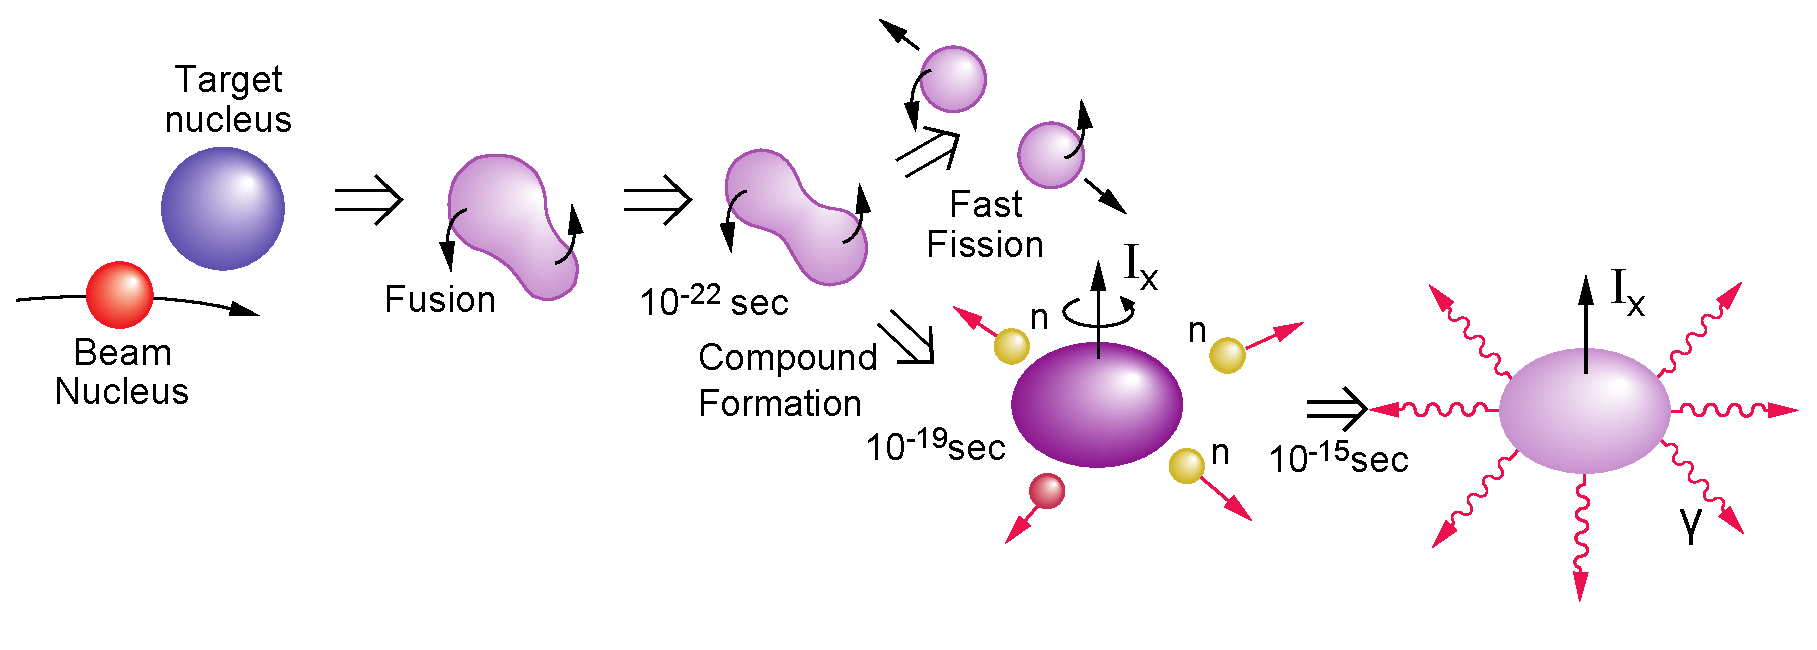
\includegraphics[width=\textwidth]{./img/c3/fusion_evaporation_horizontal.pdf}}
	\caption{Schematic illustration of heavy-ion fusion-evaporation, adapted from Ref. \cite{gsBooklet}.}
	\label{fig:chp3-fus-evap-schem}
\end{figure}

While it is possible for a compound nucleus to be formed for beam energies below the coulomb barrier the probability is dramatically lower as the beam must quantum mechanically tunnel through the barrier. Therefor for use of heavy ion fusion to be experimentally feasible the center of momentum energy must exceed the height of the coulomb barrier. The coulomb barrier height can be estimated with \ref{eqn:cb_en} and the non-relativistic limit the center of momentum energy is given in Eqn. \ref{eqn:cmf_en} (for the relativistic formula see Appendix \ref{app:rel-kin}). 

\begin{equation}
\label{eqn:cb_en}
E_{CB}=\frac{\alpha \hbar c Z_b Z_t}{1.16 fm (A_b^{1/3} + A_t^{1/3} + 2)}
\end{equation}

\begin{equation}
\label{eqn:cmf_en}
E_{cm} = \frac{A_{b}}{A_{b}+A_{t}}E_{b}
\end{equation}

Here the subscripts $b$ and $t$ denote beam and target respectively, $A$ is the mass number, $Z$ represents the nuclear charge, and $\alpha{}$ is the fine structure constant. 

\subsection{Choice of Beam and Target}
\label{ssec:exp-pr-fus-evap-beam-target}
When choosing the beam and target for a fusion evaporation one must find the best compromise for 
\subsubsection{Channel Selection}
\label{sssec:exp-pr-fus-evap-beam-target-channel}
\subsubsection{PACE4}
\label{sssec:exp-pr-fus-evap-beam-pace4}

\section{Gamma-ray Spectroscopy}
\label{sec:exp-pr-gamma-spec}
\subsection{Gamma-ray Interaction with Matter}
\label{ssec:exp-pr-gamma-spec-interactions}
\subsection{High Purity Germanium (HPGe) Detectors}
\label{ssec:exp-pr-gamma-spec-hpge}
\subsection{Escape Suppression with BGO detectors}
\label{ssec:exp-pr-gamma-spec-escape-supress}
\subsection{Gammasphere}
\label{ssec:exp-pr-gamma-gammasphere}
\subsection{Indian National Gamma Array (INGA)}
\label{ssec:exp-pr-gamma-spec-inga}

\section{Experimental Details}
\label{sec:exp-pr-details}
\subsection{ATLAS/Gammasphere}
\label{ssec:exp-pr-details-gs}
\subsection{TIFR - BARC Pelletron LINAC / INGA}
\label{ssec:exp-pr-details-inga}

\section{Data Processing}
\label{sec:exp-pr-data-proc}
\subsection{Calibration}
\label{ssec:exp-pr-data-proc-cal}
\subsection{Background Subtraction}
\label{ssec:exp-pr-data-proc-bg-sub}
\subsubsection{Symmetric Gates}
\label{sssec:exp-pr-data-proc-bg-sub-sym}
\subsubsection{Asymmetric Gates}
\label{sssec:exp-pr-data-proc-bg-sub-asym}

\section{Angular Distributions, Correlations, and Polarization}
\label{sec:exp-pr-data-ang}
\subsection{Angular Distributions}
\label{ssec:exp-pr-data-ang-dist}
Testing 1
\subsection{Angular Correlations}
\label{ssec:exp-pr-data-ang-cor}
Testing 2
\subsubsection{Directional Correlation of Gamma-rays from Oriented Nuclei DCO Ratios}
\label{sssec:exp-pr-data-ang-cor-dco}
Testing 3
\subsection{Polarization}
\label{ssec:exp-pr-data-ang-pol}
Testing 4
